\section{Challenges in XAI} \label{sec:Challenges}

Feature relevancy with saliency maps are a popular method of interpreting the decisions of DNNs, but methods for generating these saliency maps may be manipulated with adversarial inputs.  Given a set of feature saliency maps from a DNN, it is possible to create an iterative optimizer that can take an intended input into the DNN and a target feature saliency map and generates an adversarial input that is indiscernible to the human eye \cite{DBLP:journals/corr/abs-1812-00891}.  The iterative optimizer perturbs the original input based on the target feature saliency map and bound by a perturbation magnitude so that the internals of the DNN may be computed in such a way that a similar response is achieved while the explanation of the decision has been manipulated.  This method of adversarial attack on feature relevance analysis on a DNN requires the adversary to have obtained previous feature saliency maps from the DNN and also the ability to inject an adversarial input into the DNN.  Also, in order for the attack to have value, it must occur in a context in which the analysis of feature relevancy is occurring.  These constraints limit the feasibility and value of this type of attack on real-time systems, but as seen in figure \ref{fig:zhang2018}, the result of this type of attack can have a significant observable impact.

\begin{figure}
    \centering
    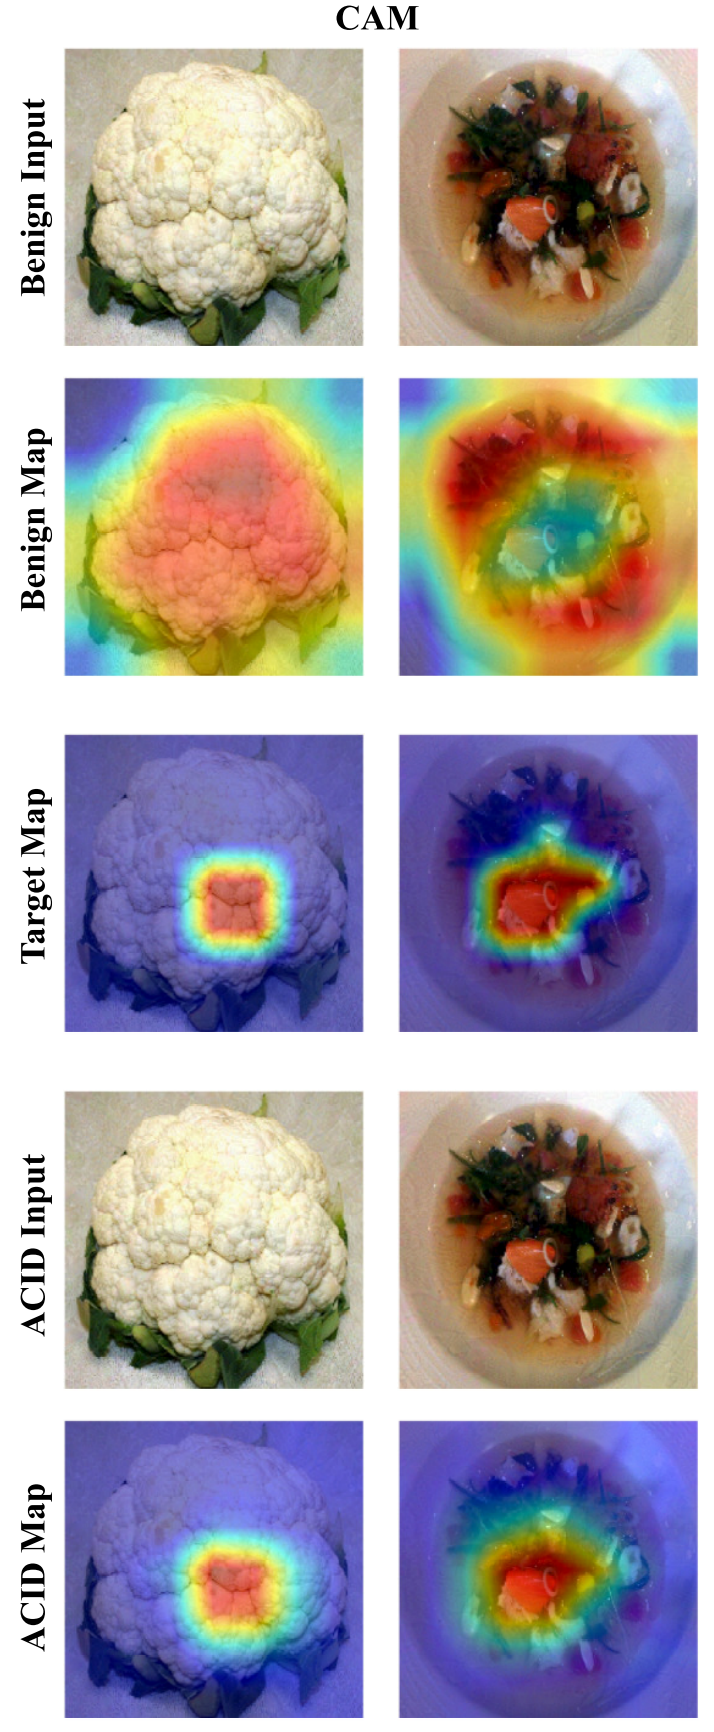
\includegraphics[height=7in]{media/zhang2018.png}
    \caption{Zhang et al. create adversarial inputs to deceive a DNN in attributing feature relevance based on a target map \cite{DBLP:journals/corr/abs-1812-00891}}.
    \label{fig:zhang2018}
\end{figure}

The interpretation of responses from machine learning models are subjective and rely on the user's intuition.  The vocabulary around the field of XAI is not yet mature or homogenous, creating rifts in how researchers describe problems and approach the study of human interpretability in machine learning.  Related terms in research include the study of comprehensibility and understandability, and the study of these topics can be contextualized around the concepts of interestingness, usability, acceptability, and justifiability \cite{Bibal2016}.  Quantitative characteristics of models are also studied for their impact on interpretability, such as the size of a model's feature input or topology \cite{Bibal2016}.  There is a lack of literature that relates the measures and concepts of interpretability to specific methods of XAI.

Stakeholders of automated decision systems cover a wide variety of backgrounds with differing domain knowledge, intentions of participation, and access to interfacing with the system.  An explanation for expert users may provide little to no value to lay users, such as owners and consumers.  Some ML systems, such as autonomous vehicle and facial recognition software, may be deployed in public settings in which the data subjects had no knowing participation in the ML system's decision making process.  The General Data Protection Regulation (GDPR) provides a right for consumers to access the data of theirs that companies collect \cite{Mittelstadt2017}, but designing the systems and interfaces for such a wide audience of stakeholders is a complicated challenge.

Even if methods of XAI may be applied effectively, in practice, the auditing and accounting of automated decision systems in private industry is rife with tedium, complicated legacy systems, and noncooperation \cite{Veale:2018:FAD:3173574.3174014}.  It is difficult for researchers to study the application of XAI in practice unless there is internal motivation for the owners of the ML process to do so because a private organization is at risk at being exposed for implementing, likely unintentionally, biased or unfair decision systems.  While it is popular anecdote that machine learning systems are replacing legacy, human-driven analytics in droves, these legacy analytic processes are steeped in cultural domain knowledge in the organization which does not fit succinctly into the XAI methods that have been developed via academic experimentation \cite{Veale:2018:FAD:3173574.3174014}.  The implementation of XAI methods in practice in private organizations is an uphill battle.
